O primeiro passo para verificar se a frequência natural de uma máquina está assumindo um valor coerente com a aplicação é comparando-a com a frequência de operação dela. Dessa forma, utilizando uma frequência de operação de 30 MHz --- proveniente dos motores e definida nas especificações de projeto, é preciso garantir que a frequência natural de vibração da solução seja maior que essa. 


Dada a complexidade da estrutura detalhada e da definição de uma equação do movimento que poderia ser proveniente da situação real das guias e das mesas, será utilizado um modelo de simplificação, com algumas hipóteses assumidas. O livro \cite{blevins2001formulas} foi utilizado como base para definição desse modelo estrutural para este cálculo. Assim, a versão simplificada do elemento crítico vibrante --- guia e mesa --- foi considerada como uma barra esbelta com uma massa apoiada no centro. Duas alterativas foram consideradas, representadas na Fig. \ref{fig:blevins-models}.

\begin{figure}[h]
    \centering
    \begin{subfigure}{0.45\textwidth}
         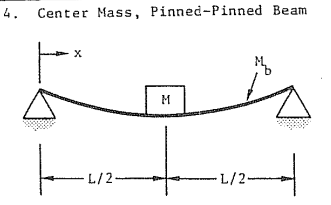
\includegraphics[width=\textwidth]{images/frequencia/center-mass-pinned-pinned.png}
         \caption{Viga bi-apoaiada}
    \end{subfigure}
    \begin{subfigure}{0.45\textwidth}
         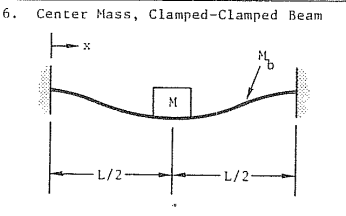
\includegraphics[width=\textwidth]{images/frequencia/center-mass-clamped-clamped.png}
         \caption{Viga bi-engastada}
    \end{subfigure}
    \caption{Modelos de viga esbelta com massa central. Fonte: \cite{blevins2001formulas}}
    \label{fig:blevins-models}
\end{figure}

Para o modelo representado em \ref{fig:blevins-models}(a), a frequência natural pode ser sintetizada pela Eq. \ref{eq:pinned-pinned}, enquanto o modelo em \ref{fig:blevins-models}(b) pela Eq. \ref{eq:clamped-clamped}.

\begin{equation}
\frac{2}{\pi}\left[\frac{3EI}{L^3 (M+0.49M_b)}\right]^{1/2}
\label{eq:pinned-pinned}
\end{equation}

\begin{equation}
\frac{4}{\pi}\left[\frac{3EI}{L^3 (M+0.37M_b)}\right]^{1/2}
\label{eq:clamped-clamped}
\end{equation}

Considerando o pior caso, em que a frequência natural de vibração é menor e, pontanto, mais próxima da frequência mínima limitada pelas especificações do projeto, foi selecionado o modelo da Eq. \ref{eq:pinned-pinned}: a viga bi-apoiada. 

Uma vez selecionado o modelo, é possível estudar a expressão para que sejam especificados os parâmetros utilizados. Destrinchando-os, é preciso conhecer propriedades mecânicas, esturturais e geométricas dos elementos da composição --- guias e a massa móvel:
\begin{itemize}
    \item  E --- módulo de elasticidade do perfil 
    \item I --- segundo momento de inércia do perfil quando uma carga é aplicada e ha deflexão
    \item L --- comprimento do perfil 
    \item M --- massa móvel posicionada no centro do perfil
    \item $M_b$ --- massa dos perfis/guias
\end{itemize}

Adicionalmente, é possível detalhar o momento de inércia  e a massa móvel, definindo-os respectivamente a partir das Eqs. \ref{eq:inertia} e \ref{eq:movel}. O momento de inércia é como o momento de inércia a flexão para duas barras cilíndricas, no caso do eixo das guias. Como a seção é formada for duas barras, deve-se multiplicar o valor de $I$ por dois. Vale ressaltar que esse cálculo pode ser aplicado para as soluções convencionais onde a seção mais propensa a vibração por flexão é a das guias lineares. Posteriormente, na análise de cada uma das soluções, são propostos cálculos de momentos de inércia e massas móveis específicas para cade um dos modelos.  

\begin{equation}
 I = \frac{\pi R^4}{4} 
\label{eq:inertia}
\end{equation}


\begin{dmath}
    M_{\text{móvel}} = (\text{Massa da mesa deslizante})\times 2 + \text{Massa dos perfis da mesa superior} + \text{Massa do porta ferramenta}
\label{eq:movel}
\end{dmath}


A partir dessas expressões, é necessário fornecer o valor de mais parâmetros, sendo eles:
\begin{itemize}
    \item R --- raio dos perfis
    \item $\rho$ --- massa específica do material que compõe o perfil e a mesa (nessa aplicação, esse material é aço)
\end{itemize}


Dessa maneira, é possível determinar, baseado no posicionamento e na escolha das mesa deslizantes assim como sua fixação e adição de massas móveis, qual será a frequência crítica de vibração natural. 

Em adição, é também possível determinar outro tipo de frequência natural de vibração, sendo ela a vibração torsional, que pode ocorrer entre as guias e a mesa. Mas, como essa seria menos menos crítica em relação á frequência de operação, não será limitante para este projeto. 

% de aço = 200 ∗ 109P a
% • L : Comprimento do perfil = 430 ∗ 10−3m
% • Lmesa4 : Comprimento do perfil = 280 ∗ 10−3m
% • R : Raio dos perfis = 10 ∗ 10−3m
% • ρ : massa espec´ıfica a¸co = 7870kg/m3
% • Mb : Massa dos perfis = 2.13kg
% • M : Massa m´ovel = 10.5kg
% • d : distˆancia at´e o eixo = 36 ∗ 10−3m




%% maior rigidez e a da torre -> precisamos determinar a rigidez dele 




%% Frequencia torsional 




% A frequência máxima que vai ser atingida por nossa máquina é 30Hz.(Motores)
% Considerando a rigidez das estruturas das soluções apresentadas, pode-se constatar que os suportes com perfil quadrado em aço de 100mm e 80 mm apresentam um momento de inércia superior ao do perfil da barra delgada da mesa deslizante número 3 que possui 430 mm de comprimento e dois perfis cilíndricos de 20 mm de diâmetro, com um momento de inércia inferior.
% Dessa forma, calculou-se a frequência natural para a mesa deslizante 3 considerando os suportes apresentados nas soluções, biapoiados, e uma massa concentrada no meio dos perfis cilíndricos que corresponde a mesa deslizante de
% número 4, 280 mm, o porta-ferramenta, motor de passo e demais chapas de aço.

